% This is "sig-alternate.tex" V2.0 May 2012
% This file should be compiled with V2.5 of "sig-alternate.cls" May 2012
%
% This example file demonstrates the use of the 'sig-alternate.cls'
% V2.5 LaTeX2e document class file. It is for those submitting
% articles to ACM Conference Proceedings WHO DO NOT WISH TO
% STRICTLY ADHERE TO THE SIGS (PUBS-BOARD-ENDORSED) STYLE.
% The 'sig-alternate.cls' file will produce a similar-looking,
% albeit, 'tighter' paper resulting in, invariably, fewer pages.
%
% ----------------------------------------------------------------------------------------------------------------
% This .tex file (and associated .cls V2.5) produces:
%       1) The Permission Statement
%       2) The Conference (location) Info information
%       3) The Copyright Line with ACM data
%       4) NO page numbers
%
% as against the acm_proc_article-sp.cls file which
% DOES NOT produce 1) thru' 3) above.
%
% Using 'sig-alternate.cls' you have control, however, from within
% the source .tex file, over both the CopyrightYear
% (defaulted to 200X) and the ACM Copyright Data
% (defaulted to X-XXXXX-XX-X/XX/XX).
% e.g.
% \CopyrightYear{2007} will cause 2007 to appear in the copyright line.
% \crdata{0-12345-67-8/90/12} will cause 0-12345-67-8/90/12 to appear in the copyright line.
%
% ---------------------------------------------------------------------------------------------------------------
% This .tex source is an example which *does* use
% the .bib file (from which the .bbl file % is produced).
% REMEMBER HOWEVER: After having produced the .bbl file,
% and prior to final submission, you *NEED* to 'insert'
% your .bbl file into your source .tex file so as to provide
% ONE 'self-contained' source file.
%
% ================= IF YOU HAVE QUESTIONS =======================
% Questions regarding the SIGS styles, SIGS policies and
% procedures, Conferences etc. should be sent to
% Adrienne Griscti (griscti@acm.org)
%
% Technical questions _only_ to
% Gerald Murray (murray@hq.acm.org)
% ===============================================================
%
% For tracking purposes - this is V2.0 - May 2012

\documentclass{sig-alternate}

\begin{document}
%
% --- Author Metadata here ---
\conferenceinfo{MediaEval}{'15 Wurzen, Germany}
%\CopyrightYear{2007} % Allows default copyright year (20XX) to be over-ridden - IF NEED BE.
%\crdata{0-12345-67-8/90/01}  % Allows default copyright data (0-89791-88-6/97/05) to be over-ridden - IF NEED BE.
% --- End of Author Metadata ---

\title{MediaEval 2015: Retrieving Diverse Social Images with Image Search for Result Diversification}
\subtitle{[Can I discard this?]
%\titlenote{A full version of this paper is available as
%\textit{Author's Guide to Preparing ACM SIG Proceedings Using
%\LaTeX$2_\epsilon$\ and BibTeX} at
%\texttt{www.acm.org/eaddress.htm}}}
%
% You need the command \numberofauthors to handle the 'placement
% and alignment' of the authors beneath the title.
%
% For aesthetic reasons, we recommend 'three authors at a time'
% i.e. three 'name/affiliation blocks' be placed beneath the title.
%
% NOTE: You are NOT restricted in how many 'rows' of
% "name/affiliations" may appear. We just ask that you restrict
% the number of 'columns' to three.
%
% Because of the available 'opening page real-estate'
% we ask you to refrain from putting more than six authors
% (two rows with three columns) beneath the article title.
% More than six makes the first-page appear very cluttered indeed.
%
% Use the \alignauthor commands to handle the names
% and affiliations for an 'aesthetic maximum' of six authors.
% Add names, affiliations, addresses for
% the seventh etc. author(s) as the argument for the
% \additionalauthors command.
% These 'additional authors' will be output/set for you
% without further effort on your part as the last section in
% the body of your article BEFORE References or any Appendices.

\numberofauthors{2} %  in this sample file, there are a *total*
% of EIGHT authors. SIX appear on the 'first-page' (for formatting
% reasons) and the remaining two appear in the \additionalauthors section.
%
\author{
% You can go ahead and credit any number of authors here,
% e.g. one 'row of three' or two rows (consisting of one row of three
% and a second row of one, two or three).
%
% The command \alignauthor (no curly braces needed) should
% precede each author name, affiliation/snail-mail address and
% e-mail address. Additionally, tag each line of
% affiliation/address with \affaddr, and tag the
% e-mail address with \email.
%
% 1st. author
\alignauthor
Shiran Dudy\\\
       \affaddr{Center for Spoken Language Understanding}\\
       \affaddr{OHSU}\\
       \affaddr{Portland, Oregon}\\
       \email{dudy@ohsu.edu}
% 2nd. author
\alignauthor
Steven Bedrick\\\
       \affaddr{Center for Spoken Language Understanding}\\
       \affaddr{OHSU}\\
       \affaddr{Portland, Oregon}\\
       \email{bedricks@ohsu.edu}
}

\date{20 Agoust 2015}
% Just remember to make sure that the TOTAL number of authors
% is the number that will appear on the first page PLUS the
% number that will appear in the \additionalauthors section.

\maketitle
\begin{abstract}
These working notes will describe the motivation, process, results and 
analysis of results that the we have worked on as part of the 
MediaEval task of `The 2015 Retrieving Diverse Social Images Task'. 
The concept of our approach was in implementing a technique \cite{fscore} borrowed from documents retrieval field 
and applying it to the image domain with appropriate adjustments. 
The core idea here was that the decision making process, to produce the ranked image sequence, 
was done iteratively. Determining how different and relevant an image in 
the stack is relatively to the already chosen images. 

\end{abstract}

\keywords{Information Retrival, Image Retrieval, Diversity function, Relevance, Ranked list}

\section{Introduction}
Imagine you are in Munich and it's just about time that everybody around you talks about going to 
Oktoberfest. Being unfamiliar with this festival you are about to search for it to understand better if 
you'd like this event and what to expect. The task of this year's MediaEval 2015 was to provide the most
diverse and relevant images to describe a place or an event in a spesific place given a query like Oktoberfest.
The organizers provided us with a fully detailed task description alnog with data set for development and test 
found in \cite{mediaEval2015}.


\section{Related Work}
%To try answering this question the task 
%orginizers provided data along with task description that are found in \cite{mediaEval2015}
The task of ordering images in a search engine given a query is
still a developing field.  The focus of this
task is on retrieving diverse and relevant images from a given set of images.
The motivation to our approach was based on a recent paper \cite{fscore} that 
described an iterative scoring method for both relevance and diversity of 
a textual document. Every document was scored against the documents that were already 
chosen. The scoring function is described in Eq.~\ref{eq:process}:
\begin{equation}
f_{s}(x_{i},R_{i})=w_{r}^{T}\mathbf{x_{i}+}w_{d}^{T}h_{s}(R_{i}),\forall x_{i}\in X\backslash S\label{eq:process}
\end{equation}
The scoring function combines information on relevance and diversity given the candidate document $x_{i}$ and its
diversity matrix $R_{i}$. 
While the prediction part above scores and chooses images the training part's purpose is
to produce the relevance and diversity weight vectors $w_{r}$, $w_{d}$ that are used in Eq.~\ref{eq:process}.
%The \textit{proceedings} are the records of a conference.
%ACM seeks to give these conference by-products a uniform,
%high-quality appearance.  To do this, ACM has some rigid
%requirements for the format of the proceedings documents: there
%is a specified format (balanced  double columns), a specified
%set of fonts (Arial or Helvetica and Times Roman) in
%certain specified sizes (for instance, 9 point for body copy),
%a specified live area (18 $\times$ 23.5 cm [7" $\times$ 9.25"]) centered on
%the page, specified size of margins (1.9 cm [0.75"]) top, (2.54 cm [1"]) bottom
%and (1.9 cm [.75"]) left and right; specified column width
%(8.45 cm [3.33"]) and gutter size (.83 cm [.33"]).



\section{The Method}
Our task's objective is to utilize the scoring concept for images while incorporating the necessary tools to determine an image scoring function. In our task 
the relevence feature vector $\mathbf{x_{i}}$ was composed of Latent Semantic Analysis (LSA) \cite{lsa} of `tags' and `description' textual fields, 
information on the user's credibility of `visualScore', 1-`faceproportion', `tagSpecificity', `uniqueTags', 1-`locationSimilarity', and 1-`bulkProportion', 
and the normalized numerical data of image features.
The diversity feature vector $h_{s}(R_{i})$ was composed of the following features with their coresponding distance metrics: 
`tags' and `description' textual fields with cosinedisimilarity, this fields were used with Latent Dirichlet Allocation(LDA) \cite{lda} for topic diversity, `csd' with l2 distance \cite{csd}, `hog' with Batacharia distance \cite{hog}, 1cn' with
euclidian distance \cite{cn}, `cm' with Canberra distance \cite{cm}, `lbp' with Chisquare distance \cite{glbp}, `glr' with l1 distance \cite{glr}, 
and `cnn' with Mahalanobis distance \cite{cnn}. A feature represent a more relevant or diverse as higher its value gets.
The three algorithms described in \cite{fscore} were reduced to two algorithms since queries were provided with ranked lists 
of relevance.


\subsection{Settings}
Settings that remained similar across experiments were:
in relevance feature vector: user credibility information, lsa on `tag' an `description', and in diversity feature vector:
lda on `tag' an `description', `hog' and `csd'.
We implemented four different settings:
\newline 1) f1 - is using the global image features (without `cnn')
\newline 2) f2 - is using the local image features (without `cnn')
\newline 3) f1r f2d cnn - is using the global image features for relevance, local for diversity and global 'cnn'
\newline 4) f2 cnn2 - is using the local image features with local `cnn'


\section{Results}
Apart from reporting the official results we would first like to show the development set results of 
two experiments: f1 and f2. These were computed seperately to the official results. We divided devset to 10-1 train test ratio
and trained. Both f1 and f2 were trained and tested on same sets which were exclusice. 
Table~\ref{tab:dev} has the results of both experiments:

\begin{table}[t]
\noindent \begin{centering}
\subfloat{\noindent \protect\centering{}%
\begin{tabular}{l|c|c|c}
 & F-score & RC & P\tabularnewline
\hline 
f1 Dev & 0 & 0 & 0\tabularnewline
f2 Dev & 0.43 & 0.31 & 0.75\tabularnewline
\end{tabular}\protect}
\par\end{centering}

\protect\caption{\label{tab:dev}Development set results.}
\end{table}
2) train, prediction, exp

graphs of the small set


\begin{figure}
\centering
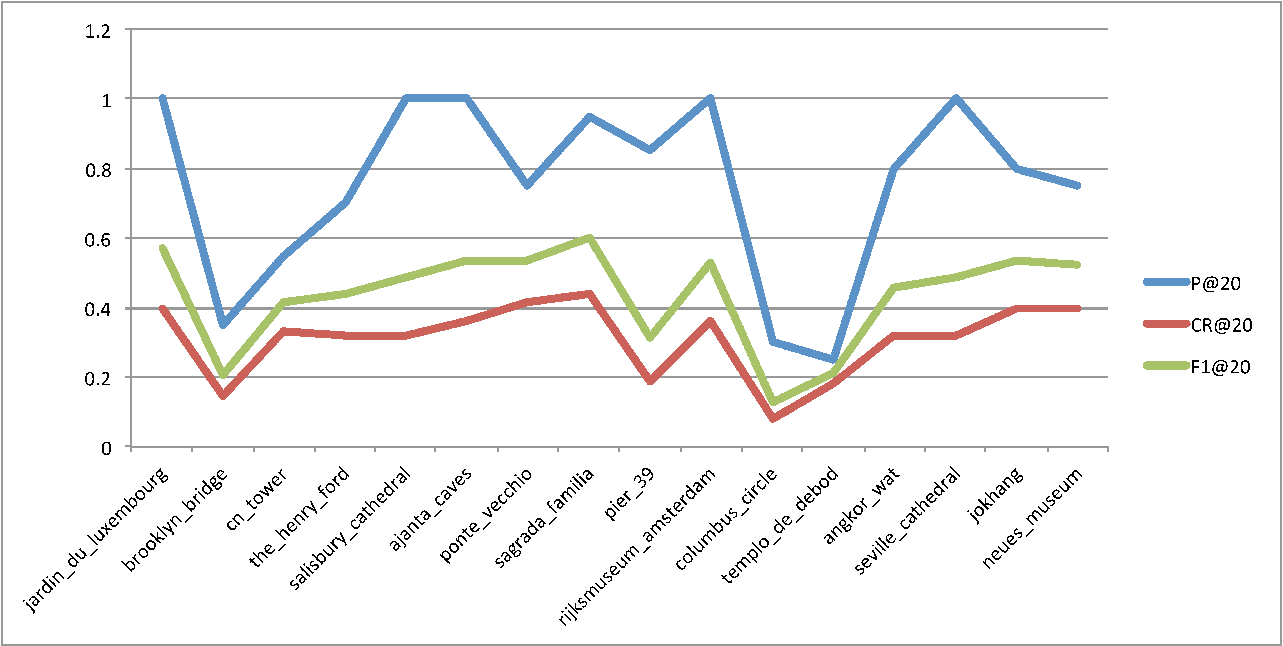
\psfig{file=dev2.ps, height=1.75in, width=3in,}
\caption{F-score, precision and coverage rates of f2 development.}
\vskip -6pt
\end{figure}



\section{Conclusions}
This paragraph will end the body of this sample document.
Remember that you might still have Acknowledgments or
Appendices; brief samples of these
follow.  There is still the Bibliography to deal with; and
we will make a disclaimer about that here: with the exception
of the reference to the \LaTeX\ book, the citations in
this paper are to articles which have nothing to
do with the present subject and are used as
examples only.
%\end{document}  % This is where a 'short' article might terminate


%
% The following two commands are all you need in the
% initial runs of your .tex file to
% produce the bibliography for the citations in your paper.
\bibliographystyle{abbrv}
\clearpage\bibliography{references}  % sigproc.bib is the name of the Bibliography in this case
% You must have a proper ".bib" file
%  and remember to run:
% latex bibtex latex latex
% to resolve all references
%
% ACM needs 'a single self-contained file'!
%
%APPENDICES are optional
%\balancecolumns

\end{document}
